\documentclass[gra_conf.tex]{subfiles}
\begin{document}

\begin{figure}[h]
  \centering{
  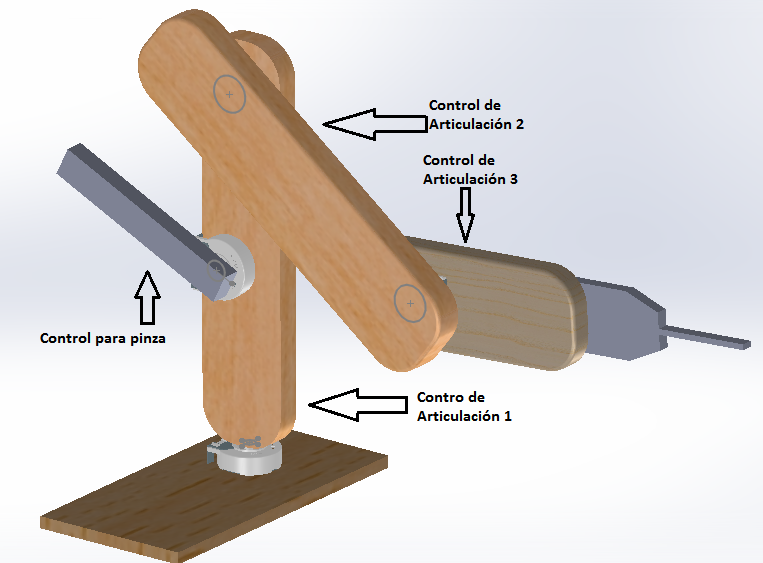
\includegraphics[width=0.3\textwidth]{../img/Replica1.png}
  \caption{Brazo a escala - perspectiva 1}
  \label{brazo_replica1}
  }
\end{figure}

Se puede observar en la imagen 3.1 los sistemas mecánicos para realizar
el control del brazo robótico. En cada articulación se encuentra un 
potenciómetro, el cual cambiará su resistencia en función del ángulo
en el  que se gire cada eslabón. Los eslabones forman una réplica del
brazo robótico, a excepción de la pequeña palanca, la cual funcinará
como control de la pinza.

\begin{figure}[h]
  \centering
  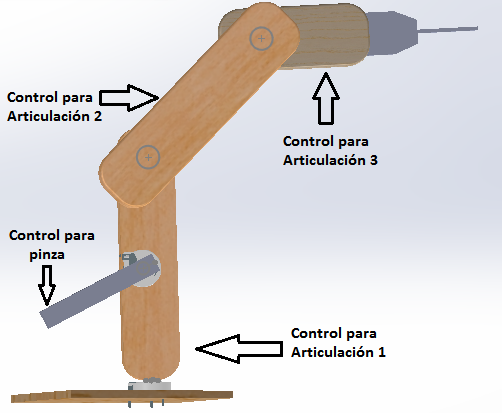
\includegraphics[width=0.3\textwidth]{../img/Replica2.png}
  \caption{Brazo a escala - perspectiva 2}
  \label{brazo_replica2}
\end{figure}

Cada potenciómetro va conectado a una entrada analógica de un Arduino UNO, 
con la cual, junto con un muestreo previo, se podrá aproximar el ángulo del 
potenciómetro, y así, se controlará las articulaciones (1, 2, 3, pinza) del 
robot. Se pueden observar las partes de la réplica en la Fig. 3.2.

\begin{figure}[h]
  \centering
  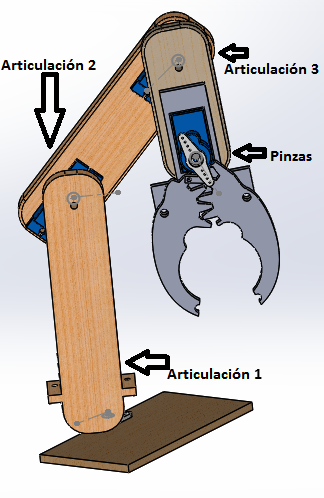
\includegraphics[width=0.2\textwidth]{../img/Brazo1.png}
  \caption{Brazo robótico - perspectiva 1}
  \label{brazo1}
\end{figure}

Se puede observar el chasis del robot en la Fig. 3.3. Cada articulación
tiene $180^\circ$ de amplitud de movimiento en ángulo, debido a que se 
usan servomotores de $90^\circ$.

El brazo posee tres articulaciones rotativas, a las cuales se les aplicó el algoritmo de Denavit - Hartemberg para definir sistemas de coordenadas en cada articulación, y finalmente poder saber, en función a los ángulos de rotación, la ubicación del extremo del brazo robótico.

Después del aplicar el algoritmo de Denavit - Hartenberg, obtenemos la siguiente tabla de parámetros:


\begin{tabular}[t]{|c|c|r| r| r|}
           \hline
		1 & \theta_1 & 0 & 8.9 & 90\\
	\hline
		2 & \theta_2 & 6.6 & 0 & 0\\
	\hline
		3 & \theta_3 & 5.6 & 1.9 & 0\\
	\hline
\end{tabular}


Se puede usar la matriz de transformación para estimar la posición final de la pinza en función de ángulos de giro de cada servomotor dado:

\centering{
c(\theta_i) = cos(\theta_i)

s(\theta_i) = sin(\theta_i)

A_{i+1}^{i}=
\[
	\left[
		\begin{array}{lcrh}
			c(\theta_i) & -c(\alpha_i) s(\theta_i) & s(\theta_i) s(\alpha_i) & a_i c(\theta_i)\\
			s(\theta_i) & c(\theta_i) c(\alpha_i) & -s(\alpha_i) c(\theta_i) & a_i s(\theta_i) \\
			0 & s(\alpha_i) & c(\alpha_i) & d_i \\
			0 & 0 & 0 & 1 \\
		\end{array}
	\right]
\]
}

La matriz de transformación del sistema de coordenadas base, al sistema de coordenadas de la pinza es:

\centering
T_{4}^{0} = A_{3}^{2}A_{2}^{1}A_{1}^{0}


\begin{figure}[h]
\centering
  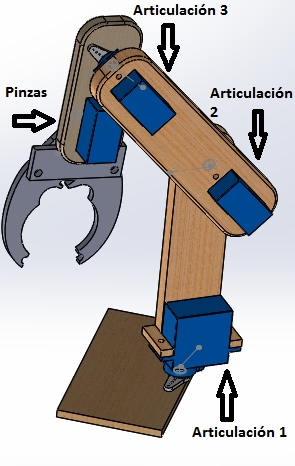
\includegraphics[width=0.2\textwidth]{../img/Brazo2.png}
  \caption{Brazo robótico - perspectiva 2}
  \label{brazo2}
\end{figure}

\end{document}